\documentclass{beamer}
\usetheme{default}

\title{Algorithms for numerical solution of initial value problems}
\author{Chris Williams, Jonathan Heathcote, Karl Sutt, Matt Leach, Thomas Nixon}

\begin{document}

\begin{frame}
	\titlepage
\end{frame}
\begin{frame}{Question 1}

$y_{n+3} + (2b - 3)(y_{n+2} - y_{n+1}) - y_n = hb(f_{n+2} + f_{n+1}), b \in \Re$

Method stability determined by roots of first characteristic polynomial of magnitude $\le 1$ with values of b.

${\it y_{n+3}}+\left(2\,b-3\right)\,{\it y_{n+2}}+\left(3-2\,b\right) {\it y_{n+1}}-{\it y_n}$

Giving alphas: $\alpha_3 = 1$ $\alpha_2 = 2b - 3$ $\alpha_1 = 3 - 2b$ $\alpha_0 = -1$

Which gives us the first characteristic polynomial:

$\rho(\xi) = \xi^3+\left(2\,b-3\right)\,\xi^2+\left(3-2\,b\right)\,\xi-1$

Factorizing gives: $\left(\xi-1\right)\,\left(\xi^2+2\,b\,\xi-2\,\xi+1\right)$

Root at $\xi = 1$. Quadratic formula gives the roots:

$\left[ \xi=-\sqrt{b^2-2\,b}-b+1 , \xi=\sqrt{b^2-2\,b}-b+1 , \xi=1 \right]$

The interval of values for the real constant b for which the method is stable is $0 < b < 2$
\end{frame}

\begin{frame}{Question 2}

A linear multistep method is of order p if:

$$C_0 = C_1 = ... = C_p = 0, C_{p+1} \ne 0$$

Constants to check for equality to 0:
\begin{align*}
C_0 &= \alpha_0 + \alpha_1 + \alpha_2 + \alpha_3\\
C_1 &= \alpha_1 + 2\alpha_2 + 3\alpha_3 - (\beta_0 + \beta_1 + \beta_2 + \beta_3)\\
	C_j &= \frac{1}{j!} (\alpha_1 + 2^j\alpha_2 + 3^j\alpha_3) - \frac{1}{(j-1)!} (\beta_1 + 2^{j-1}\beta_2 + 3^{j-1}\beta_3)
\end{align*}

\end{frame}

\begin{frame}{Question 2}
Using:\\
$$\Sigma_{i=0}^{k}\alpha_iy_{n+i} = h \Sigma_{i=0}^{k} \beta_i f_{n+i}, n=0,1,\ldots$$

Gives alphas:
\begin{align*}
\alpha_3 &= 1\\ 
\alpha_2 &= 2b - 3\\
\alpha_1 &= -(2b - 3)\\
\alpha_0 &= -1
\end{align*}

And betas:
\begin{align*}
\beta_3 &= 0\\
\beta_2 &= b\\
\beta_1 &= b\\
\beta_0 &= 0
\end{align*}

\end{frame}

\begin{frame}{Question 2}
Calculate the constants
\begin{align*}
C_0 &= -1 - (2b - 3) + (2b - 3) + 1 = 0\\
C_1 &= -(2b - 3) + 2(2b-3) + 3 - 2b = 0\\
C_2 &= \frac{1}{2}(-(2b-3) + 4(2b-3) + 9) - 3b = \frac{1}{2} (6b - 9 + 9) - 3b = 0\\
C_3 &= \frac{1}{6}[-(2b-3) + 8(2b-3) + 27] - \frac{1}{2}(b+4b)\\
    &= \frac{1}{6}[7(2b-3) + 27] - \frac{1}{2}5b = \frac{14b}{6} + 1 - \frac{5b}{2}\\
    &= 1 - \frac{b}{6} \ne 0, \texttt{for } b \in (0,2)
\end{align*}

So,
$$p = 2$$

\end{frame}

\begin{frame}{Question 3}

%Using Euler's method to compute the first 'n' initial values can 
%introduce a lot of error into the solution. A better method would be to 
%calculate the next point by Euler's and then the next point with the 
%generic IVP solution for order two and so on until we have the correct 
%initial number of values.

For $t_1$:

\begin{align*}
t_1 &= t_0 + h_E = h_E\\
y_{1,1} &= h_E(\mu - \beta (h_E)y_{1,0}y_{3,0}) + y_{1,0}\\
y_{2,1} &= h_E\left(\beta (h_E)y_{1,0}y_{3,0} - \frac{1}{\lambda}y_{2,0}\right) + y_{2,0}\\
y_{3,1} &= h_E\left(\frac{1}{\lambda}y_{2,0} - \frac{1}{\eta}y_{3,0} \right ) + y_{3,0}\\
\end{align*}

If we had numbers, we should now solve these three equations to get numerical answer for $y_{1,1}$ $y_{2,1}$ and $y_{3,1}$

\end{frame}

\begin{frame}{Question 3}

For $t_2$:

\begin{align*}
t_2 &= 2h_E\\
y_{1,2} &= h_E(\mu - \beta (h_E)y_{1,0}y_{3,0}) + y_{1,0} + (\mu - \beta(2h_E)y_{1,0}y_{3,0})h_E\\
y_{2,2} &= h_E\left(\beta (h_E)y_{1,0}y_{3,0} - \frac{1}{\lambda}y_{2,0}\right) + y_{2,0} + h_E\left(\beta (2h_E)y_{1,0}y_{3,0} - \frac{1}{\lambda}y_{2,0}\right)\\
y_{3,2} &= h_E\left(\frac{1}{\lambda}y_{2,0} - \frac{1}{\eta}y_{3,0} \right ) + y_{3,0} + h_E\left(\frac{1}{\lambda}y_{2,0} - \frac{1}{\eta}y_{3,0} \right )\\
\end{align*}

Again we should solve these equations simultaneously to $y_{1,2}$ $y_{2,2}$ and $y_{3,2}$.


\end{frame}

\begin{frame}{Question 4}
	\begin{center}
		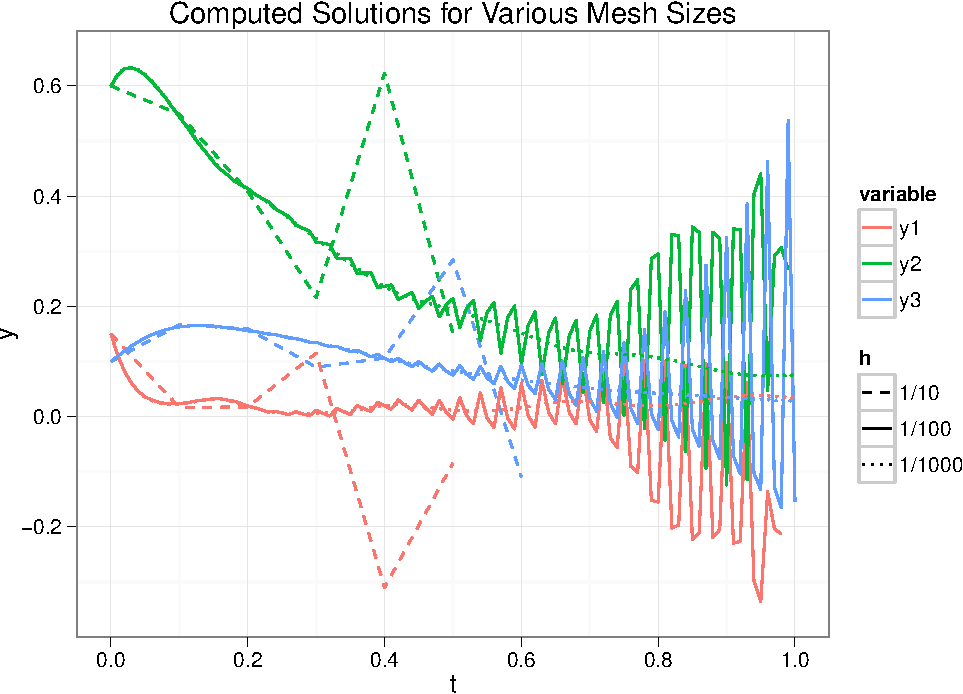
\includegraphics[width=\textwidth]{plot-crop.pdf}
	\end{center}
\end{frame}

\begin{frame}{Question 4}
	\begin{center}
		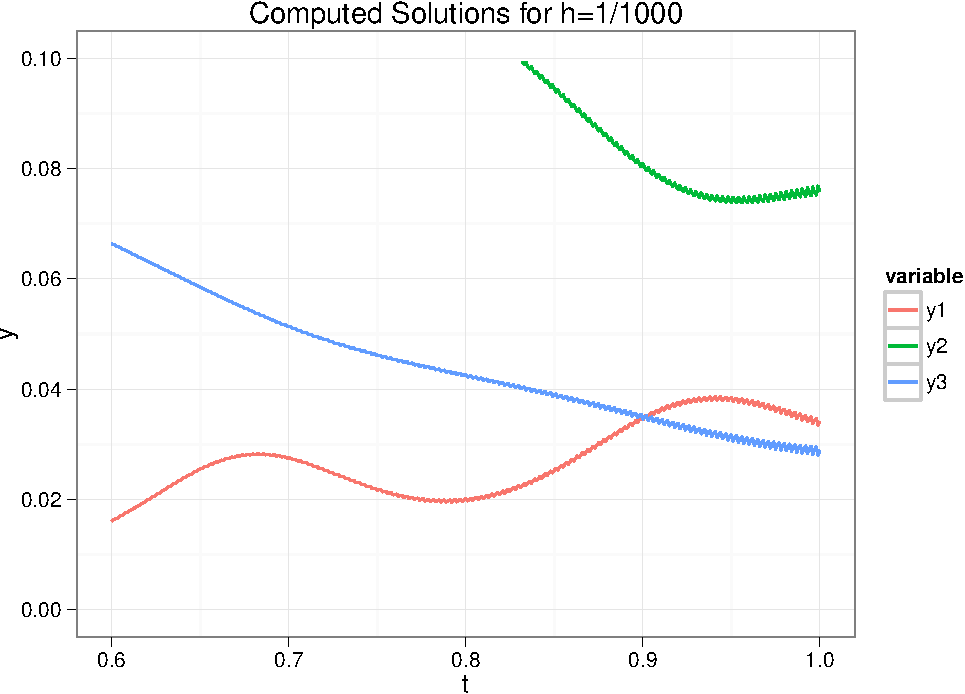
\includegraphics[width=\textwidth]{plot-small-crop.pdf}
	\end{center}
\end{frame}

\end{document}
